%%==================================================================%%
%% Author : Abascal Fern�ndez, Patricia                             %%
%%          S�nchez Barreiro, Pablo                                 %%
%% Version: 1.3, 17/04/2013                                         %%
%%                                                                  %%
%% Memoria del Proyecto Fin de Carrera                              %%
%% Antecedentes, archivo ra�z                                       %%
%%==================================================================%%

\chapterheader{Antecedentes}{Antecedentes}
\label{chap:background} 

Este cap�tulo trata de describir a grandes rasgos las t�cnicas, tecnolog�as y herramientas utilizadas para el desarrollo del presente Proyecto Fin de Carrera. En primer lugar, se introducir� el caso de estudio que se utilizar� de forma recurrente a lo largo del proyecto, que es una l�nea de productos software para software de control para hogares inteligentes. Para ello se describen en primer lugar diversos conceptos relacionados el dominio del proyecto, como son las l�neas de productos software, la tecnolog�a TENTE, el dise�o orientado a caracter�sticas, el patr�n slicer y la generaci�n de c�digo.
\chaptertoc

\section{Caso de Estudio: Software para Hogares Inteligentes}
\label{sec:back:casoEstudio}

%%==================================================================%%
%% Author : Abascal Fern�ndez, Patricia                             %%
%%          S�nchez Barreiro, Pablo                                 %%
%% Version: 1.1, 17/04/2013                                         %%
%%                                                                  %%
%% Memoria del Proyecto Fin de Carrera                              %%
%% Planificacion/CasoEstudio                                        %%
%%==================================================================%%

El objetivo �ltimo del presente proyecto es la construcci�n de una l�nea de productos software sobre la plataforma .NET para hogares automatizados y/o inteligentes.

El objetivo de estos hogares es aumentar la comodidad y seguridad de sus habitantes, as� como hacer un uso m�s eficiente de la energ�a consumida. Los ejemplos m�s comunes de tareas automatizadas dentro de un hogar inteligente son el control de las luces, ventanas, puertas, persianas, aparatos de fr�o/calor, as� como otros dispositivos, que forman parte de un hogar. Un hogar inteligente tambi�n busca incrementar la seguridad de sus habitantes mediante sistemas automatizados de vigilancia y alerta de potenciales situaciones de riesgo. Por ejemplo, el sistema deber�a encargarse de detecci�n de humos o de la existencia de ventanas abiertas cuando se abandona el hogar.

El funcionamiento de un hogar inteligente se basa en el siguiente esquema: (1) el sistema lee datos o recibe datos de una serie de sensores; (2) se procesan dichos datos; y (3) se activan los actuadores para realizar las  acciones que correspondan en funci�n de los datos recibidos de los sensores.

Todos los sensores y actuadores se comunican a trav�s de un dispositivo especial denominado puerta de enlace (\emph{Gateway}, en ingl�s). Dicho dispositivo se encarga de coordinar de forma adecuada los diferentes dispositivos existentes en el hogar, de acuerdo a los par�metros y preferencias especificados por los habitantes del mismo. Los habitantes del hogar se comunicar�n con la puerta de enlace a trav�s de una interfaz gr�fica.
Este proyecto tiene como objetivo el desarrollo de un hogar inteligente como una l�nea de productos software, con un n�mero variable de plantas y habitaciones. El n�mero de habitaciones por planta es tambi�n variable. La l�nea de productos deber� ofrecer varios servicios, que podr�n ser opcionalmente incluidos en la instalaci�n del software para un un hogar determinado. Dichos servicios se clasifican en funciones b�sicas y complejas, las cuales describimos a continuaci�n.

\paragraph{Funciones b�sicas} \ \\

\begin{enumerate}
\item \emph{Control autom�tico de luces:} Los habitantes del hogar deben ser capaces de encender, apagar y ajustar la intensidad de las diferentes luces de la casa. El n�mero de luces por habitaci�n es variable. El ajuste debe realizarse especificando un valor de intensidad.
\item \emph{Control autom�tico de ventanas:} Los residentes tienen que ser capaces de controlar las ventanas autom�ticamente. De tal modo que puedan indicar la apertura de una ventana desde las interfaces de usuario disponibles.
\item \emph{Control autom�tico de persianas:} Los habitantes podr�n subir y bajar las persianas de las ventanas de manera autom�tica.
\item \emph{Control autom�tico de temperatura:} El usuario ser� capaz de ajustar la temperatura de la casa. La temperatura se medir� siempre en grados celsius.
\end{enumerate}

\paragraph{Funciones complejas} \ \\

\begin{enumerate}
\item \emph{Control inteligente de energ�a:} Esta funcionalidad trata de coordinar el uso de ventanas y aparatos de fr�o/calor para regular la temperatura interna de la casa de manera que se haga un uso m�s eficiente de la energ�a. Por ejemplo, si se recibe la orden de calentar la casa, a la vez que se activan los radiadores se cerrar�n las ventanas para evitar las p�rdidas de calor.
\item \emph{Presencia simulada:} Para evitar posibles robos, cuando los habitantes abandonen la casa por un periodo largo de tiempo, se deber� poder simular la presencia de personas en las casas. Hay dos opciones de simulaci�n (no exclusivas):
	\begin{enumerate}
	\item \emph{Simulaci�n de las luces:} Las luces se deber�n apagar y encender para simular la presencia de habitantes en la casa.
	\item \emph{Simulaci�n de persianas:} Las persianas se deber�n subir y bajar autom�tica para simular la presencia de individuos dentro de la casa.
	\end{enumerate}
\end{enumerate}

Todas estas funciones son opcionales. Las personas interesadas en adquirir el sistema podr�n incluir en una instalaci�n concreta de este software el n�mero de funciones que ellos deseen. La siguiente secci�n profundiza en el concepto \emph{l�nea de productos software}. 

\section{L�neas de Producto Software}
\label{sec:back:spl}

%%==================================================================%%
%% Author : Abascal Fern�ndez, Patricia                             %%
%%          S�nchez Barreiro, Pablo                                 %%
%% Version: 1.3, 18/06/2013                                         %%
%%                                                                  %%
%% Memoria del Proyecto Fin de Carrera                              %%
%% Background/Software Product Lines                                %%
%===================================================================%%

El objetivo de una \emph{l�nea de producto software}~\citep{pohl:2010,kakola:2006} es crear una infraestructura adecuada a partir de la cual se puedan derivar, de forma tan autom�tica como sea posible, producto concretos pertenecientes a una familia de producto software. Una familia de producto software es un conjunto de aplicaciones software similares, lo que implica que comparten una serie de caracter�sticas comunes, pero que tambi�n presentan variaciones entre ellos.

Un ejemplo cl�sico de familia de producto software es el producto Parten�n, para software bancario, comentado en la introducci�n a este documento (ver Secci�n~\ref{sec:intr:introduction}). Dicho producto representa una familia de productos destinados a la gesti�n bancaria. Parten�n en s� no puede ser desplegado como una aplicaci�n, sino que necesita ser configurado de acuerdo a una serie de caracter�sticas concretas demandadas por cada cliente que require una instalaci�n de Parten�n.

La idea de una l�nea de producto software es proporcionar una forma autom�tica y sistem�tica de construir productos concretos dentro de una familia de producto software mediante la simple especificaci�n de qu� caracter�sticas deseamos incluir dentro de dicho producto. Esto representa una alternativa al enfoque tradicional de desarrollo software, el cual se basaba simplemente en seleccionar el producto m�s parecido, dentro de la familia, al que queremos construir y adaptarlo manualmente.

El proceso de creaci�n de l�neas de producto software se estructura dos fases: (1) \emph{Ingenier�a del Dominio} (en ingl�s,  \emph{Domain Engineering}); y (2) \emph{Ingenier�a de Aplicaci�n} (en ingl�s, \emph{Application Engineering}) (ver Figura~\ref{back:fig:domainAplicEng}). La \emph{Ingenier�a del Dominio} tiene como objetivo la creaci�n de la infraestructura o arquitectura de referencia de la l�nea de productos software. Esta arquitectura de referencia debe permitir la r�pida, o incluso autom�tica, construcci�n de sistemas software espec�ficos pertenecientes a la familia de productos software. La \emph{Ingenier�a de Aplicaci�n} utiliza la infraestructura creada anteriormente para crear aplicaciones espec�ficas adaptadas a las necesidades de cada usuario en concreto.

\begin{figure}[!tb]
  \centering
  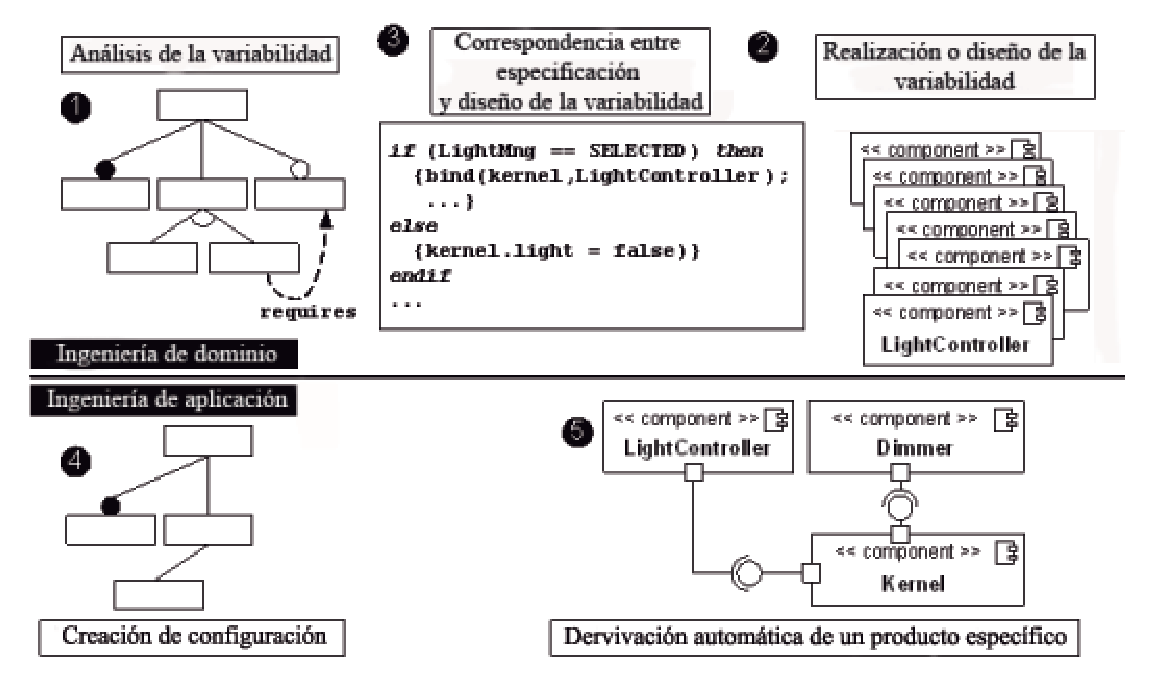
\includegraphics[width=.95\linewidth]{background/images/domainAplicationEngineering.eps} \\
  \caption{Proceso de Desarrollo de una l�nea de producto software}
  \label{back:fig:domainAplicEng}
\end{figure}

En la fase de Ingenier�a del Dominio, el primer paso a realizar es un an�lisis de qu� caracter�sticas de la familia de producto son variables y por qu� son variables. Esta parte es la que se conoce como \emph{An�lisis o Especificaci�n de la Variabilidad} (Figura~\ref{back:fig:domainAplicEng}, etiqueta 1).

A continuaci�n, se ha de dise�ar una arquitectura de referencia para la familia de producto software que permita soportar dicha variabilidad. Esta actividad se conoce como \emph{Realizaci�n o Dise�o de la Variabilidad} (Figura~\ref{back:fig:domainAplicEng}, etiqueta 2).

El siguiente paso es establecer una serie de reglas que especifiquen c�mo hay que instanciar o configurar la arquitectura previamente creada de acuerdo con las caracter�sticas seleccionadas por cada cliente. Esta fase es la que se conoce como \emph{Correspondencia entre Especificaci�n y Dise�o de la Variabilidad} (Figura~\ref{back:fig:domainAplicEng}, etiqueta 3).

Tras completar la fase de Ingenier�a del Dominio, disponemos de una especie de l�nea de montaje, la cual podemos utilizar para construir productos concretos de forma m�s o menos automatizada.

En la fase de Ingenier�a de Aplicaci�n, se crean productos concretos utilizando la infraestructura previamente creada. Para ello, el primer paso es crear una \emph{configuraci�n}, que no es m�s que una selecci�n de caracter�sticas que un usuario desea incluir en su producto concereto (Figura~\ref{back:fig:domainAplicEng}, etiqueta 4).

En el caso ideal, usando esta configuraci�n, se debe poder ejecutar las reglas de correspondencia entre especificaci�n y dise�o de la variabilidad para que la arquitectura creada en la fase de Ingenier�a del Dominio se adapte autom�ticamente; generando un producto concreto espec�fico acorde a las necesidades concretas del usuario (Figura~\ref{back:fig:domainAplicEng}, etiqueta 5). En el caso no ideal, dichas reglas de correspondencia deber�n ejecutarse a mano, lo cual suele ser un proceso tedioso, largo, repetitivo y propenso a errores.

La siguiente secci�n describe el paradigma de desarrollo software orientada a caracter�sticas, el cual est� �ntimamente ligado al dise�o e implementaci�n de l�neas de productos software.



\section{TENTE}
\label{sec:back:tente}

%%==================================================================%%
%% Author : Abascal Fernández, Patricia                             %%
%%          Sánchez Barreiro, Pablo                                 %%
%% Version: 1.0, 15/04/2013                                         %%
%%                                                                  %%
%% Memoria del Proyecto Fin de Carrera                              %%
%% Background/TENTE                               %%
%===================================================================%%

TENTE~\cite{fuentes:2009:caise,sanchez:2011:tente} es una moderna metodología para el desarrollo de líneas de productos software desarrollada en el contexto del proyecto AMPLE\footnote{www.ample-project.net}. TENTE integra diversos avances para el desarrollo de líneas de productos software, tales como avanzadas técnicas de modularización y desarrollo software dirigido por modelos.

Las técnicas avanzadas de modularización permiten el encapsulamiento en módulos bien definidos y fácilmente componibles de las diferentes características de una familia de productos software, lo cual simplifica el proceso de construcción de productos específicos. Dicha modularización de características se realiza desde la fase arquitectónica, usando mecanismos específicos del lenguaje de modelado UML~\cite{uml:2005}. Después, mediante el uso de generadores de código, a partir del diseño arquitectónico de una familia de productos software se genera el esqueleto de su implementación. Dicha implementación se realiza en el lenguaje CaesarJ~\cite{aracic:2006}, una extensión de Java que incluye potentes mecanismos para soportar la separación y composición de características. Dichos esqueletos se completan manualmente, obteniéndose al final un conjunto de módulos software, o piezas, cuya composición da lugar a productos software concretos\footnote{El nombre de la metodología proviene del célebre juego de construcción TENTE, versión española del popular Lego.}. Esta fase constituye la definición de la infraestructura desde la cual se derivarán los productos concretos.

Para la derivación de productos concretos desde la infraestructura descrita en el párrafo anterior, TENTE usa
un innovador lenguaje, denominado VML~\cite{loughran:2008,sanchez:2008}, basado en transformaciones de modelo a modelo de orden superior. Dicho lenguaje sirve para especificar qué acciones hay que realizar sobre un modelo que describe la familia completa de productos software para adaptarlo a las necesidades del cliente. Posteriormente, dada una lista con las características que el cliente desea incluir o excluir de su producto concreto, VML es capaz de transformar automáticamente el modelo de la familia de productos software para adaptarlo a las necesidades de dicho cliente.

Acto seguido, se utiliza dicho modelo de un producto concreto como entrada para un generador automático de código, que creará el código necesario para componer los módulos o piezas software que se constituyeron durante la creación de la infraestructura de la línea de productos software.

Esta metodología posee diversas ventajas:

\begin{enumerate}
	\item Gracias al uso de técnicas orientadas a características, como el operador \emph{merge} de UML y el lenguaje CaesarJ, se facilita la modularización y composición de características, lo que facilita no sólo el proceso de obtención de productos concretos, sino también la reutilización y evolución de dichas características~\cite{figueiredo:2008}.
	\item Gracias al uso de técnicas dirigidas por modelos, se automatiza gran parte del proceso, evitando tareas repetitivas, largas, tediosas y monótonas, usualmente propensas a errores.
	\item Gracias al uso de lenguajes avanzados (como VML) y tecnologías estándares de modelado (como UML) se evita que los desarrolladores, tanto de la infraestructura como de los productos concretos, tengan que poseer cierta experiencia en el uso de técnicas de desarrollo software dirigido por modelos tales como creación de transformaciones de modelo a modelo en lenguajes como ATL~\cite{joault:2008} o Epsilon~\cite{kolovos:2008}.
\end{enumerate}

No obstante, a pesar de sus bondades, se han encontrado diversas dificultades a la hora de transferir esta metodología a las empresas de desarrollo software situadas en el entorno cántabro. Las principales dificultades provienen de dos fuentes distintas pero relacionadas, descritas a continuación.

\paragraph{Problema 1: Resistencia a cambiar el lenguaje de implementación habitual} \ \\

En primer lugar, y éste no es un solo un problema encontrado en el entorno de Cantabria, TENTE está basado en el uso del lenguaje CaesarJ como lenguaje de implementación. Podría usarse, con el coste asociado de tener que escribir nuevos generadores de código, lenguajes similares a CaesarJ tales como ObjectTeams~\cite{herrman:2002}. En cualquier caso, hace falta un lenguaje con fuerte soporte para la modularización y composición de características, y en especial, con soporte para \emph{clases virtuales}~\cite{madsen:1989}. La mayoría de las empresas son bastante reticentes a cambiar su lenguaje habitual de programación, debido fundamentalmente a dos motivos:

\begin{enumerate}
\item El coste de aprendizaje que ello supone, ya que los programadores han de familiarizarse con nuevos conceptos y técnicas de codificación software.
\item El uso de un nuevo lenguaje de programación podría dejar obsoletas muchas herramientas, como suites para la ejecución de casos de prueba, que la empresa podría tener asociadas al anterior lenguaje de programación.
\end{enumerate}

Además, en el caso de lenguajes de reciente creación como CaesarJ u ObjectTeams, aunque los compiladores están completamente desarrollados y son bastante estables, las facilidades auxiliares asociadas a un lenguaje de programación maduro tipo Java o C\# no están a menudo disponibles. Por ejemplo, CaesarJ no soporta compilación incremental por el momento, por lo que un ligero cambio en el nombre de un atributo obliga a recompilar el proyecto completo.

\paragraph{Problema 2: Obligatoriedad de usar la plataforma .NET} \ \\

Debido a diferentes razones estratégicas de negocio, la mayoría de las empresas de desarrollo software en Cantabria trabajan casi en exclusiva sobre la plataforma .NET~\cite{chappell:2006}, siendo además bastante reticentes a considerar el cambio a otras plataformas. La mayoría de los lenguajes con fuerte soporte para orientación a características, como suele ser el caso habitual en los lenguajes académicos, están basados en Java.

Por tanto, TENTE es una tecnología llena de ventajas, pero quizás excesivamente innovadora para el momento actual. Por dicho motivo, se decidió crear una nueva metodología, basada en TENTE, pero que resultase más fácilmente transferible a la industria. Para favorecer dicha transferencia, se tomaron dos decisiones estratégicas:

\begin{enumerate}
	\item El lenguaje de programación usado en el nivel de implementación tenía que ser un lenguaje comercial estándar, tipo Java, C\# o C++. Esto evitaría los problemas derivados de obligar a las empresas a aprender un nuevo lenguaje y estilo de programación, y sobre todo, a cambiar sus entornos de desarrollo.
	\item El nuevo lenguaje de programación de la metodología debía ser C\#~\cite{fons:2008}, al ser éste el lenguaje bandera de la plataforma .NET, y al desarrollar las empresas del entorno de nuestra universidad casi en exclusiva software para dicha plataforma.
\end{enumerate}

Tal nueva metodología recibiría el nombre de TENTE.NET (versión para la plataforma .NET de la metodología TENTE), y está actualmente en fase de desarrollo. El primer paso para la adaptación de la metodología TENTE a la plataforma .NET era encontrar un mecanismo para simular las facilidades ofrecidas por lenguajes orientados a características dentro del lenguaje C\#. Tomando las ideas de Laguna et al~\cite{laguna:2007} como base, se pensó inicialmente que las \emph{clases parciales} proporcionadas por C\# podían ser un mecanismo adecuado para alcanzar cierto grado de desarrollo orientado a características. Sin embargo, un posterior estudio realizado por López et al~\cite{elio:2010} demostraba que las clases parciales de C\# poseían más limitaciones de las inicialmente previstas por Laguna et al para la implementación de diseños software orientados a características.

Por tanto, el siguiente paso hacia la construcción de la variante para .NET de la metodología TENTE era la solución de tales limitaciones. 

Para solventar dichas limitaciones, se ideó un patrón, cuya aplicación servía para solucionar las limitaciones encontradas. En la siguiente sección se describirá el patrón utilizado para tal fin, denominado Patrón Slicer.


\section{Dise�o Orientado a Caracter�sticas con UML}
\label{sec:back:uml}

%%==================================================================%%
%% Author : Abascal Fern�ndez, Patricia                             %%
%%          S�nchez Barreiro, Pablo                                 %%
%% Version: 1.1, 17/04/2013                                         %%
%%                                                                  %%
%% Memoria del Proyecto Fin de Carrera                              %%
%% Background/Dise�o Orientado a Caracter�sticas con UML            %%
%===================================================================%%

El dise�o orientado a caracter�sticas~\cite{kastner:2008} es un paradigma para la construcci�n, adaptaci�n y s�ntesis de sistemas software a gran escala. Una caracter�stica es una unidad de funcionalidad de un sistema software que satisface un requisito, representa una decisi�n de dise�o y proporciona una opci�n de configuraci�n potencial. La idea b�sica del dise�o orientado a caracter�sticas es descomponer un sistema software en m�dulos agrupando las caracter�sticas que ofrece. El objetivo de la descomposici�n es la construcci�n de software bien estructurado que puede ser adaptado a las necesidades del usuario y al entorno de la aplicaci�n.

T�picamente, a partir de un conjunto de caracter�sticas, se pueden generar multitud de sistemas software compartiendo caracter�sticas comunes y diferenci�ndose en otras. El conjunto de los sistemas software generados a partir de un conjunto de caracter�sticas, comentado en la secci�n~\ref{sec:back:spl}, corresponde al concepto de \emph{l�nea de productos software}.

Para estudiar las ventajas del dise�o orientado a caracter�sticas nos basaremos en las facilidades proporcionadas por CaesarJ~\cite{aracic:2006}, e ilustraremos los ejemplos con diagramas UML. CaesarJ es un lenguaje de programaci�n orientado a caracter�sticas basado en Java. Para ello trabaja con el concepto de \emph{familia de clases}. Una \emph{familia de clases} es una unidad de encapsulamiento que sirve para agrupar clases relacionadas. Las familias de clases reciben un tratamiento similar al de las clases, soportando relaciones de herencia entre ellas.

Asimismo, CaesarJ tambi�n introduce el concepto de \emph{clases virtuales}. Una clase virtual es una clase perteneciente a una familia de clases y que es susceptible de ser heredada y sobreescrita por familias de clases que hereden de la familia de clases que contiene dicha clase virtual. La Figura~\ref{back:fig:caesarJExpressions} ilustra esta situaci�n. Las familias de clases se representan mediante paquetes UML, y herencia entre clases, mediante relaciones \emph{merge}. Cuando una familia de clases hereda de otra, hereda impl�citamente todas sus clases virtuales. Si la primera contiene clases virtuales con el mismo nombre que la familia de clases que hereda, entonces la clase virtual de la familia de clases hija hereda de la clase virtual con el mismo nombre de la familia de clases padre. Por ejemplo, en la Figura~\ref{back:fig:caesarJExpressions}, la clase \imp{Mult} de la familia de clases \imp{Eval} heredar�a impl�citamente de la clase \imp{Mult} de la familia de clases \imp{Basic}. En cada familia de clases hija, se pueden a�adir por tanto nuevos atributos y m�todos a las clases virtuales de las familias de clases padre. Adem�s, gracias al avanzado sistema de tipos de CaesarJ, se pueden a�adir nuevas relaciones de herencia.

\begin{figure}[ht!] 
  \centering
  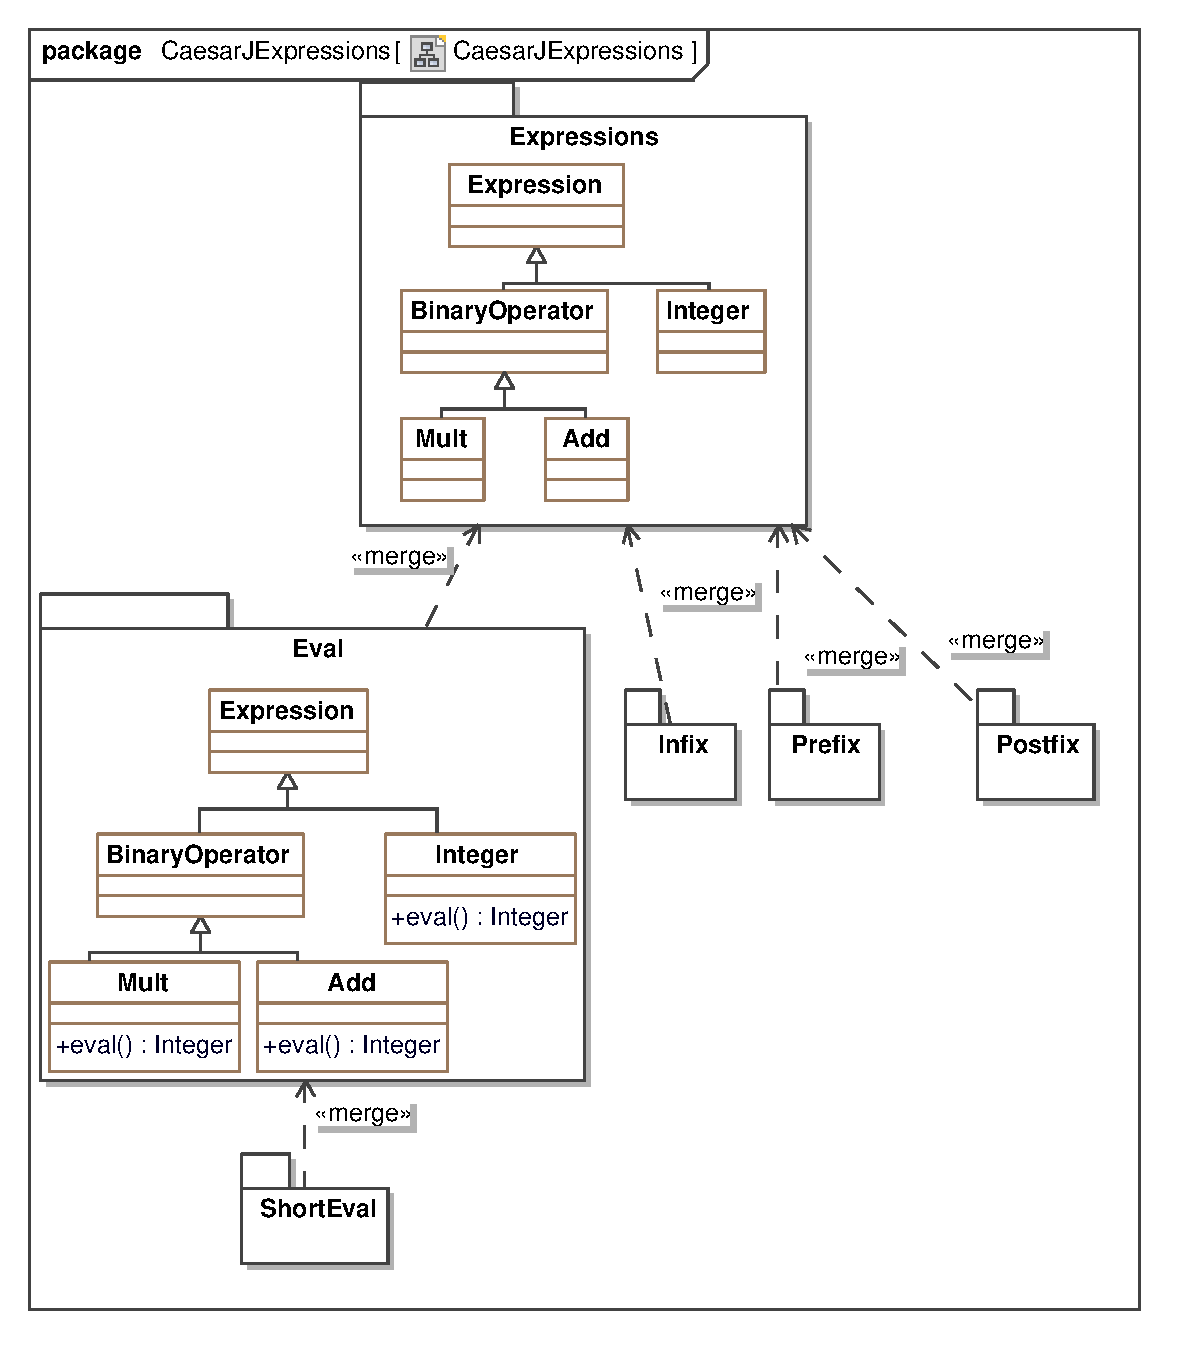
\includegraphics[width=.55\linewidth]{background/images/CaesarJExpressions.eps} \\
  \caption{Dise�o para resolver el problema de las expresiones con CaesarJ}
  \label{back:fig:caesarJExpressions}
\end{figure}

Adem�s, las referencias entre clases se actualizan autom�ticamente. Por ejemplo, en el caso de la Figura~\ref{back:fig:caesarJExpressions}, aunque no se haga expl�citamente, cualquier referencia a una clase del tipo \imp{Expression} dentro de la familia de clases \imp{Eval} se referir� a la clase virtual \imp{Expression} de la familia de clases \imp{Eval} y no a la clase virtual de mismo nombre de la familia de clases \imp{Expressions}. De esta forma, las referencias est�n siempre actualizadas a su versi�n m�s extendida.

Para implementar una l�nea de productos software, cada caracter�stica se considera como una familia de clases.
Dentro de cada familia de clases, cada caracter�stica se dise�a usando las t�cnicas tradicionales de la orientaci�n a objetos, tal como se muestra en la Figura~\ref{back:fig:caesarJExpressions}.

\begin{figure}[ht!]
  \centering 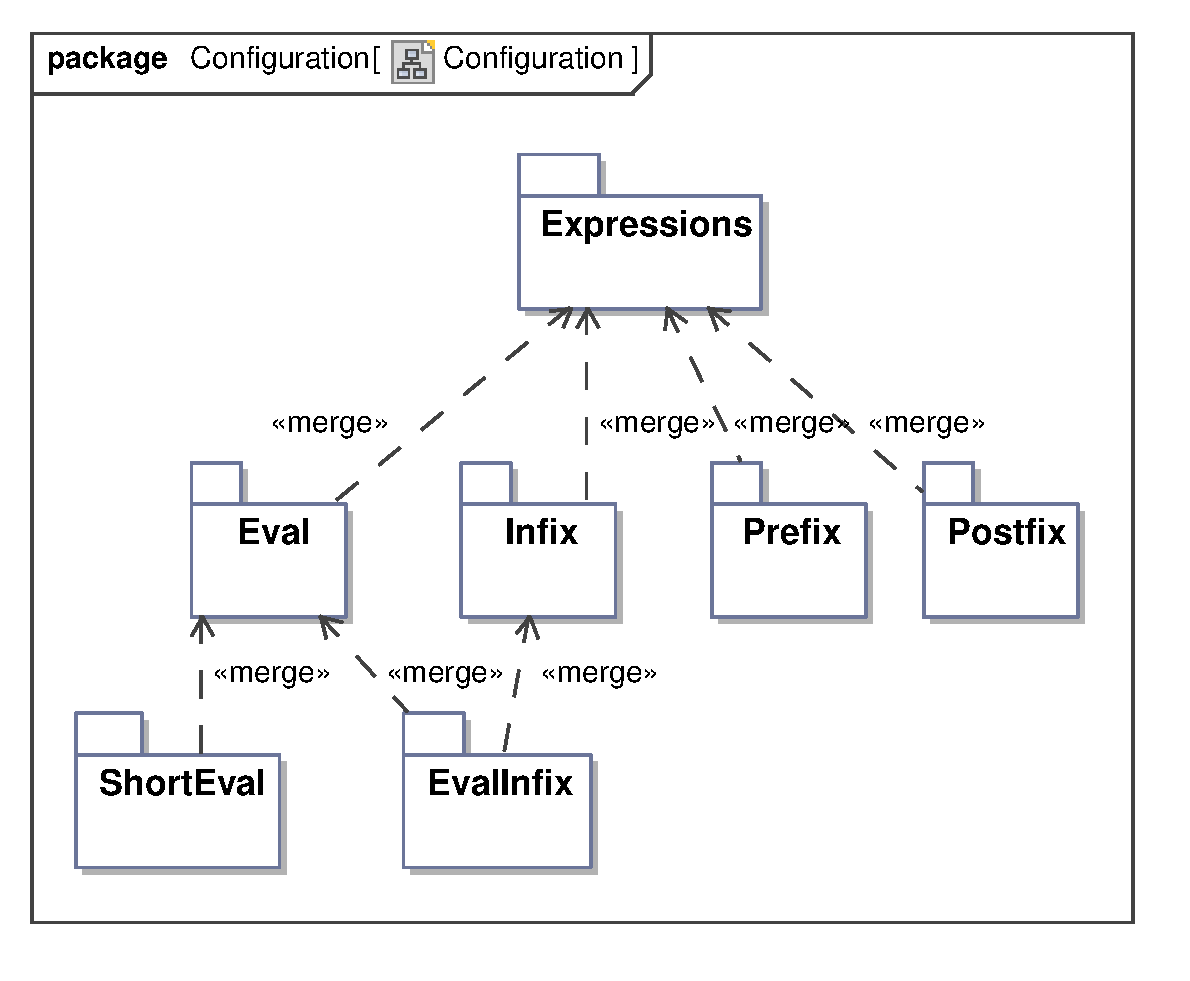
\includegraphics[width=.55\linewidth]{background/images/Configuration.eps} \\
  \caption{Composici�n de las caracter�sticas \imp{Eval} e \imp{Infix} en nuevo producto con CaesarJ}
  \label{back:fig:caesarJConfiguration}
\end{figure}

Para realizar una configuraci�n, es decir, para crear un producto concreto por composici�n de caracter�sticas, simplemente hay que crear una nueva familia de clases que herede de las familias de clases que correspondan a las caracter�sticas seleccionadas. La figura \ref{back:fig:caesarJConfiguration} muestra como se crear�a un producto nuevo mediante la composici�n de las caracter�sticas \imp{Eval} e \imp{Infix}.

Con el fin de solventar las limitaciones expuestas en la Secci�n \ref{sec:back:tente} y apoy�ndose en el dise�o orientado a caracter�sticas (Secci�n \ref{sec:back:uml}), en la siguiente secci�n se describir� el patr�n para resolver dichas limitaciones, denominado Patr�n Slicer.


\section{Slicer Pattern}
\label{sec:back:slicer}

%%==================================================================%%
%% Author : Abascal Fern�ndez, Patricia                             %%
%%          S�nchez Barreiro, Pablo                                 %%
%% Version: 1.3, 21/04/2013                                         %%
%%                                                                  %%
%% Memoria del Proyecto Fin de Carrera                              %%
%% Background/Slicer Pattern                                        %%
%===================================================================%%

Antes de proceder a la explicaci�n del Patr�n Slicer, es conveniente presentar el concepto de Clase Parcial C\# de manera breve al lector. Las clases parciales C\#~\cite{albahari:2010} permiten dividir la implementaci�n de una clase en varios archivos de c�digo fuente. Cada fragmento representa una parte de la funcionalidad global de la clase. Todos estos fragmentos se combinan en tiempo de compilaci�n para crear una �nica clase, la cual contiene toda la funcionalidad especificada en las clases parciales. Por lo tanto, las clases parciales C\# parecen un mecanismo adecuado para implementar caracter�sticas, tal como ha sido identificado por diversos autores~\cite{laguna:2007,laguna:2010}, dado que cada incremento en funcionalidad perteneciente a una caracter�stica se podr�a encapsular en una clase parcial separada. Sin embargo, las clases parciales tiene un serio inconveniente para ser utilizadas como un mecanismo de apoyo a la orientaci�n de caracter�sticas: no son compatibles con la extensi�n de m�todos ni la reescritura. El Patr�n Slicer surge como patr�n para soluci�n de esta limitaci�n.

El problema a solucionar por el Patr�n Slicer tiene su origen en el hecho de que no se puede disponer de m�todos con el mismo nombre en diferentes clases parciales.

La instanciaci�n del Patr�n Slicer~\cite{perez:2011} en los m�todos regulares, consiste en a�adir un prefijo a cada m�todo que se corresponda con el nombre de la caracter�stica a la que cada m�todo pertenece. La figura~\ref{back:fig:slicerPattern} ilustra c�mo el caso de estudio de Hogar Inteligente ha sido refactorizado siguiendo dicha idea. En esta figura, las caracter�sticas han sido representadas como rect�ngulos conteniendo clases. Cada rect�ngulo ha sido etiquetado con el nombre de la caracter�stica que representa.

\begin{figure}[!tb]
  \centering
  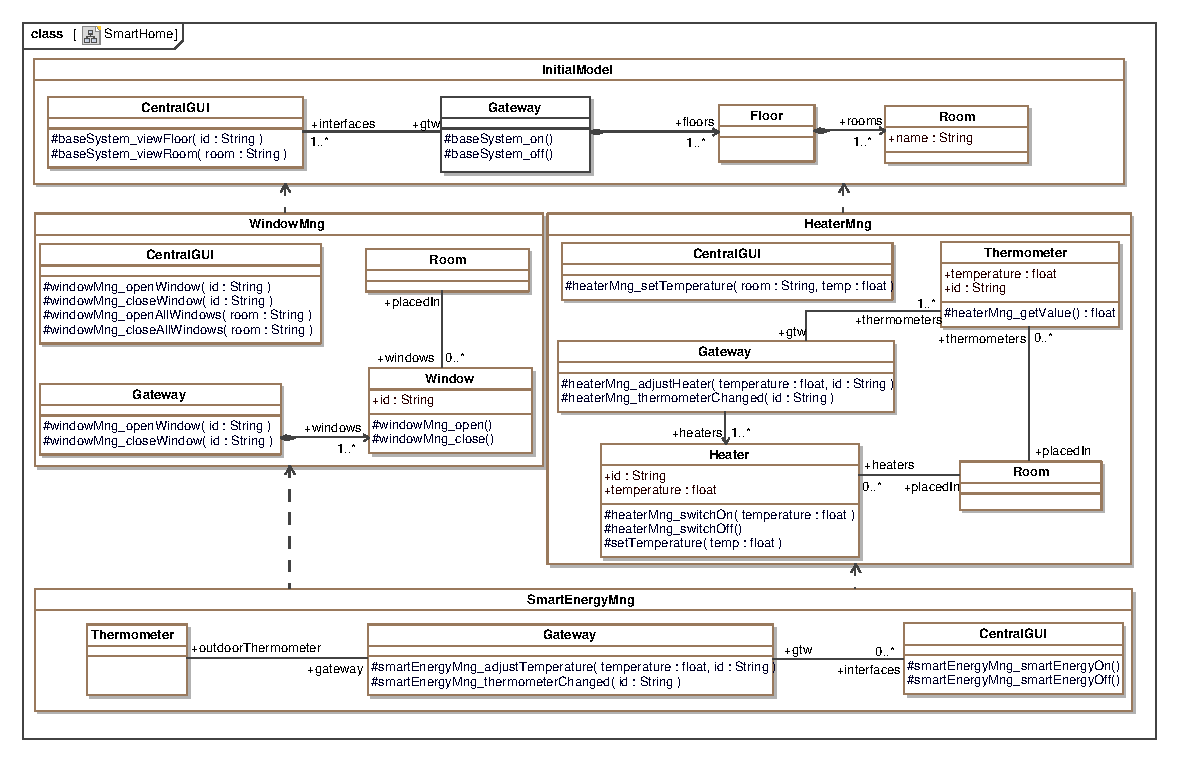
\includegraphics[width=.95\linewidth]{background/images/slicerPattern} \\
  \caption{Proceso de Desarrollo de una L�nea de Productos Software}
  \label{back:fig:slicerPattern}
\end{figure}

Usando esta estrategia se puede comprobar c�mo, por ejemplo, las versiones del m�todo \imp{thermometerChanged} correspondientes a las caracter�sticas \imp{HeaterMng} y \imp{SmartEnergyMng} han sido transformadas en \imp{heaterMng\_thermometerChanged} y \imp{smartEnergyMng\_thermometerChanged} respectivamente y por tanto pueden co-existir sin que sus nombres colisionen. Es m�s, el m�todo \imp{smartEnergyMng\_thermometerChanged} puede extender del m�todo \imp{heaterMng\_thermometerChanged}. Se dispone por tanto de varias versiones parciales de un mismo m�todo.

Para generar un producto espec�fico es necesario que, a nivel de Ingenier�a de Aplicaci�n, se cree la denominada "versi�n limpia" del m�todo \imp{thermometerChanged}, es decir, sin el prefijo. Mientras que las versiones de dicho m�todo creadas en el nivel de Ingenier�a del Dominio que han sido prefijadas con el nombre de la caracter�stica a la que cada m�todo pertenece pasar�n a ser denominadas "versiones sucias" de dicho m�todo. Adem�s, para asegurar que se invoca la versi�n correcta del m�todo, no se deber�an poder invocar los m�todos \imp{heaterMng\_thermometerChanged} y \imp{smartEnergyMng\_thermometerChanged} directamente y por dicha raz�n todas las versiones sucias de los m�todos son privadas. De dicha forma los objetos de las dem�s clases s�lo podr�n invocar a la versi�n limpia del m�todo y dicha versi�n, redireccionar� la llamada a las versiones sucias de los m�todos correspondientes de acuerdo a las caracter�sticas seleccionadas.

Sin embargo este patr�n no puede ser utilizado para los constructores de la clase ya que los constructores no se pueden renombrar porque deben tener un nombre espec�fico. De esta forma, la instanciaci�n del Patr�n Slicer en los constructores se realiza de forma diferente a la instanciaci�n del resto de m�todos. De esta forma, cada clase parcial X correspondiente a una caracter�sica F tendr� un m�todo privado llamado $<$F$>$\_init\_$<$X$>$ que contendr� el fragmento de la l�gica del constructor correspondiente a la caracter�stica F.

El listing~\ref{back:code:constSlicerPattern} muestra c�mo se aplica dicha t�cnica. Se puede apreciar c�mo la l�gica del constructor para \emph{Gateway} ha sido encapsulada en un m�todo llamado  \imp{baseSystem\_initGateway} (listing~\ref{back:code:constSlicerPattern} l�neas 03-06). La misma t�cnica ha sido usada en el listing~\ref{back:code:constSlicerPattern} l�neas 10-12 con la caracter�stica \imp{WindowMng}. El siguiente paso es encontrar un mecanismo que permita componer dichos fragmentos de acuerdo a una selecci�n de  caracter�sticas dada, de esta forma, como se puede apreciar en el listing~\ref{back:code:constSlicerPattern} l�neas 16-20, el constructor para la clase Gateway es creado con las caracter�sticas seleccionadas por el usuario final, en el caso analizado, por ejemplo, solo se ha seleccionado la caracter�stica \imp{WindowMng}.


\begin{lstlisting} [basicstyle=\ttfamily\scriptsize,language=CSharp, captionpos=b,
                    caption=C�digo para el constructor de la clase Gateway usando clases parciales y patr�n slicer,
                    label=back:code:constSlicerPattern]
File BaseSystem/Gateway.cs
--------------------------------------------------------
01 public partial class Gateway {
02      ...
03      private void BaseSystem_initGateway() {
04          this.floors = new List<Floors>();
05          this.interfaces = new List<CentralGUI>();
06      }
07 }

File WindowMng/Gateway.cs
--------------------------------------------------------
08 public partial class Gateway {
09      ...
10      private windowMng_initGateway() {
11          this.windows = new List<Window>();
12      }
13 }

File MyHouse/Gateway.cs
--------------------------------------------------------
14 public partial class Gateway {
15      ...
16      public Gateway() {
17          // WindowMng has been selected
18          baseSystem_initGateway();
19          windowMng_initGateway();
20      }
21 }
\end{lstlisting}

Concluyendo con el Patr�n Slicer, tanto los m�todos regulares como con los constructores pueden ser extendidos y reescritos usando dicho patr�n y solucionando as� las limitaciones ofrecidas por el uso de clases parciales~\cite{sanchez:2010} como mecanismo de soporte orientado a caracter�sticas. Utilizando todo lo expuesto en las secciones anteriores, en la siguiente secci�n se expone a grandes rasgos el funcionamiento de los generadores de c�digo que ser�n empleados durante la fase de Ingenier�a del Dominio del presente proyecto.


\section{Generaci�n de C�digo con Epsilon}
\label{sec:back:epsilon}

%%==================================================================%%
%% Author : Abascal Fern�ndez, Patricia                             %%
%%          S�nchez Barreiro, Pablo                                 %%
%% Version: 1.2, 18/06/2013                                         %%
%%                                                                  %%
%% Memoria del Proyecto Fin de Carrera                              %%
%% Background/Generaci�n de C�digo con Epsilon                      %%
%===================================================================%%

Epsilon~\cite{kolovos:2008} es una \emph{suite} de lenguajes y herramientas para el desarrollo software dirigido por modelos. En este sentido, Epsilon ofreces lenguajes para la transformaci�n de modelo a modelo, modelo a texto, navegaci�n a trav�s de modelos o generaci�n de editores textuales y/o gr�ficos para modelos, entre otras caracter�sticas. Epsilon se distribuye actualmente como un plug-in para Eclipse. El presente proyecto se ha centrado en la generaci�n de c�digo, para lo cual se han utilizado los lenguajes \emph{Epsilon Generation Language} (EGL)~\citep{dimitrios:2012}, que es el lenguaje de generaci�n de c�digo proporcionado por Epsilon; y \emph{Epsilon Object Language} (EOL)~\citep{dimitrios:2012}, que es el lenguaje b�sico para la manipulaci�n y navegaci�n a trav�s de modelos proporcionado por Epsilon. Describimos estos lenguajes en las siguiente subsecciones.

\subsection{Epsilon Object Language(EOL)}

El principal objetivo de EOL es proporcionar un lenguaje para la manipulaci�n a nivel de c�digo para la gesti�n de modelos. EOL proporciona facilidades para cargar un modelo, navegar a trav�s de sus elementos o leer los valores de sus elementos, entre otras cracter�sticas.

La Figura~\ref{back:code:eol} muestra un ejemplo del funcionamiento de EOL. EOL no es un lenguaje orientado a objetos en el sentido de que no permite definir clases. Sin embargo, EOL permite gestionar objetos de tipos o clases externamente definidos, normalmente dentro del metamodelo o gram�tica que define un lenguaje de modelado.

%%=======================================================================================================%%
%% [DONE]                                                                                                %%
%% NOTA(Pablo): Este ejemplo resulta demasiado sencillo. Prueba a hacer una funci�n, por ejemplo, que    %%
%%              devuelva true si una clase UML tiene m�s de un padre, es decir, est� afectada por la     %%
%%              herencia m�ltiple                                                                        %%
%%              La descripci�n es buena, haz la nueva de ese estilo                                      %%
%%=======================================================================================================%%

En la Figura~\ref{back:code:eol} l�nea 4, en este caso los objetos son de tipo Class. La l�nea 1 de la
 Figura~\ref{back:code:eol} presenta un ejemplo de llamada a operaciones EOL, donde el elemento \imp{clase}, de tipo Class, llama a la operaci�n hasParent() y devuelve, tal como se aprecia en la l�nea 9, el valor de \emph{hasParent} que ser� true o false dependiendo de si la clase a analizar presenta herencia, si es clase hija de otra clase, o no. Dicho contenido se imprime por pantalla tal como se aprecia en la l�nea 2 mediante la instrucci�n \emph{println()}).

\begin{figure}[!tb]
\begin{center}
\begin{footnotesize}
\begin{verbatim}
1 var bol = clase.hasParent();
2 bol.println();
3
4 operation Class hasParent (): Boolean{
5   var hasParent= false;
6   if (not self.generalization.isEmpty()){
7       hasParent=true;
8   }
9   return hasParent;
10 }	
\end{verbatim}
\end{footnotesize}
\end{center}
\caption{Ejemplo de operaci�n EOL}
\label{back:code:eol}
\end{figure}

De esta forma, EOL permite definir funciones auxiliares para la manipulaci�n o gesti�n de modelos. Estas funciones pueden ser utilizadas desde otros lenguajes de la suite Epsilon. En nuestro caso, estas funciones auxiliares se invocan desde el lenguaje
de transformaci�n modelo a texto EGL, el cual se describe a continuaci�n.

\subsection{Epsilon Generation Language(EGL)}

EGL es un lenguaje de transformaci�n modelo a texto (\emph{model-to-text-transformation}). EGL puede ser tulizad para transformar modelos en diversos tipos de artefactos de car�cter textual, incluyendo c�digo (por ejemplo, Java), informes (por ejemplo, en HTML), im�genes (por ejemplo, gr�ficos SVG), especificaciones formales (por ejemplo, en el lenguaje Z), o incluso aplicaciones completas generadas con m�ltiples lenguajes (por ejemplo, HTML, Javascript, CSS, Java y SQL). En nuestro caso, utilizaremos EGL para la generaci�n de c�digo C\# desde modelos UML.

EGL es un generador de c�digo basado en plantillas. Dichas plantillas son similares a las utilizadas en la generaci�n de p�ginas web din�micas, al estilo de sistemas como JSP (\emph{Java Server Pages})~\citep{eric:2010} o PHP (\emph{PHP Hypertext Preprocessor})~\citep{mehdi:2013}.

Las Figuras~\ref{back:code:generacionClases}, \ref{back:fig:epsilonEGL} y~\ref{back:code:resultadogeneracionClases} muestran un ejemplo sencillo del funcionamiento de EGL. La Figura~\ref{back:code:generacionClases} contiene una sencilla plantilla que genera un listado de las clases que contiene un modelo UML. El texto situado dentro de los caracteres de escape \texttt{[\%} y \texttt{\%]} aparecer tal cual en la salida producida por la plantilla. El c�digo situado entre dichos caracteres de escape es c�digo EGL que gobierna el proceso de generaci�n de c�digo.

Por ejemplo, las l�neas 1 y 3 declaran un bucle que recorre todas las clases contenidas en el modelo de entrada. En cada iteraci�n, se procesa la l�nea 2, que genera autom�ticamente el texto fuera de los caracteres de escape (``El modelo contiene la clase: ''). A continuaci�n, se a�ade a la salida, por medio del operador \emph{=}, el nombre de la clase \emph{c}, que corresponda con la iteraci�n realizada.

La Figura~\ref{back:code:resultadogeneracionClases} muestra el resultado que producir�a la plantilla de la Figura~\ref{back:code:generacionClases} para el modelo mostrado en la Figura~\ref{back:code:resultadogeneracionClases}.

\begin{figure}[!tb]
\begin{center}
\begin{footnotesize}
\begin{verbatim}
1 [% for (c in Class.all) { %]
2 El modelo contiene la clase: [%=c.name%]
3 [% } %]
\end{verbatim}
\end{footnotesize}
\end{center}
\caption{Generaci�n del nombre de cada Class contenida en un modelo de entrada}
\label{back:code:generacionClases}
\end{figure}

\begin{figure}[!tb]
  \centering
	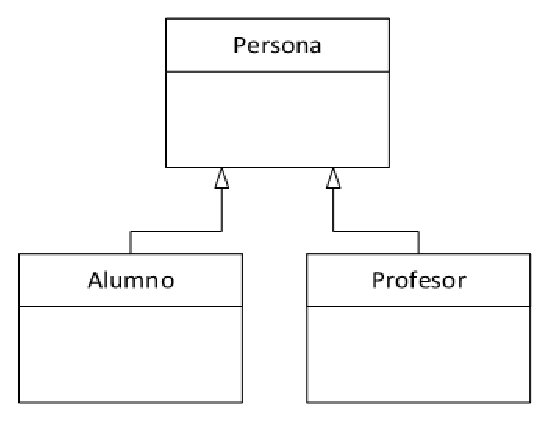
\includegraphics[width=.95\linewidth]{background/images/epsilonEGL} \\
  \caption{Ejemplo de modelo de entrada para generaci�n de c�digo con EGL}
  \label{back:fig:epsilonEGL}
\end{figure}

\begin{figure}[!tb]
\begin{center}
\begin{footnotesize}
\begin{verbatim}
1 El modelo contiene la clase: Persona
2 El modelo contiene la clase: Alumno
3 El modelo contiene la clase: Profesor
\end{verbatim}
\end{footnotesize}
\end{center}
\caption{Resultado de la generaci�n del nombre de cada Class contenida en un modelo de entrada}
\label{back:code:resultadogeneracionClases}
\end{figure}

Obviamente, EGL no s�lo nos permite realizar estas sencillas operaciones. Por ejemplo, se pueden encapsular porciones reutilizables de c�digo EGL en entidades bien definidos denominados \emph{templates}. Un \emph{template} tiene una funcionalidad similares a la de una \emph{funci�n} o \emph{procedimiento} de un lenguaje de programaci�n convencional.

La Figura~\ref{back:code:generacionOperacion} muestra un ejemplo de template que sirve para generar la cabecera de una clase Java. La cabecera del template (l�nea 2) especifica que el template de aplica a objetos del tipo \emph{Class}, no precisando de ning�n par�metro de entrada. La clase a la cual se aplica el template es un par�metro impl�cito de entrada a esta operaci�n, a la cual se puede acceder a trav�s del operador \emph{self}. Utilizando este operador, la l�nea 4 genera la cabecera de una calse java, de acuerdo a la visibilidad \emph{self.visibility} y nombre \emph{self.name} de la clase sobre la cual se invoca esta operaci�n. Siendo $c$ un objeto de tipo \emph{Class}, invocar este template ser�a tan f�cil como escribir \emph{c.getHeader()}.

\begin{figure}[tb!]
\begin{center}
\begin{footnotesize}
\begin{verbatim}
1 [% @template
2 operation Class getHeader() { %]
3 [%=self.visibility] class [%=self.name%] {}
4 [% } %]
\end{verbatim}
\end{footnotesize}
\end{center}
\caption{Ejemplo de template en EGL}
\label{back:code:generacionOperacion}
\end{figure}

Una vez explicados estos conceptos, estamos preparados para poder definir c�mo se ha estructurado y desarrollado el presente Proyecto Fin de Carrera. Dicha planificaci�n se presenta en la siguiente secci�n.

%%=====================================================================================================%%
%% NOTA(Pablo): Esto es interesante, pero se hace ya pesado, as� que yo lo quitar�a                    %%
%%=====================================================================================================%%

%Un \emph{template} proporciona tres utilidades b�sicas al desarrollador EGL:

%\begin{enumerate}
%	\item Un \emph{template} permite modularizar y reutilizar el c�digo utilizado en un proceso de transformaci�n modelo a texto.
%    \item Un \emph{template} permite al usuario definir de forma f�cil el destino del texto generado.  En la Figura~\ref{back:code:template} (l�nea 3) muestra un ejemplo de invocaci�n de un template, cuyo destino es un fichero de texto denonimado \emph{output.txt}
%     \item Y por �ltimo, proporciona un conjunto de operaciones que se usan para controlar el destino del texto generado. En la Figura~\ref{back:code:template} (l�nea 3) se muestra c�mo se elige el fichero destino para almacenar el texto generado con la plantilla \emph{ClassNames.egl}.
% \end{enumerate}

% \begin{figure}[tb!]
% \begin{center}
% \begin{footnotesize}
% \begin{verbatim}
% 1 [%
% 2 var t : Template = TemplateFactory.load("ClassNames.egl");
% 3 t.generate("Output.txt");
% 4 %]
% \end{verbatim}
% \end{footnotesize}
% \end{center}
% \caption{Almacenar el nombre de cada Class en disco}
% \label{back:code:template}
% \end{figure}




\section{Sumario}
\label{sec:back:sumario}

%===================================================================%%
%% Author : Tejedo Gonz�lez, Daniel                                 %%
%%          S�nchez Barreiro, Pablo                                 %%
%% Version: 1.0, 7/02/2013                                       %%                   
%%                                                                  %%
%% Memoria del Proyecto Fin de Carrera                              %%
%% Antecedentes, Sumario                      %%
%%==================================================================%%

Durante el cap�tulo de antecendes se han descrito los conceptos necesarios para lograr comprender el �mbito y el alcance de este proyecto, as� como el caso de estudio que se utilizar� a lo largo del documento en numerosas ocasiones y las tecnolog�as implicadas en el desarrollo de la aplicaci�n.
En el siguiente cap�tulo profundizaremos acerca del primer paso de la creaci�n de nuestro lenguaje de restricciones: la creaci�n de la sintaxis abstracta. Hablaremos con cierto nivel de detalle sobre el proceso de dise�o del metamodelo del lenguaje y sobre sus implicaciones.
